\documentclass[authoryear, review, 11pt]{elsarticle}

\setlength{\textwidth}{6.5in}
%\setlength{\textheight}{9in}
\setlength{\topmargin}{0in}
\setlength{\oddsidemargin}{0in}
\setlength{\evensidemargin}{0in}

\usepackage{amsmath}
\usepackage{amsthm}
\usepackage{amssymb}

\usepackage{bm}

%\geometry{landscape}                % Activate for for rotated page geometry
\usepackage[parfill]{parskip}    % Activate to begin paragraphs with an empty line rather than an indent
\usepackage{graphicx}
\usepackage{epstopdf}
\usepackage{natbib}

\usepackage{relsize}
\usepackage{subfigure}
%\usepackage{fullpage}
\usepackage{booktabs}

\DeclareGraphicsRule{.tif}{png}{.png}{`convert #1 `dirname #1`/`basename #1 .tif`.png}
\DeclareMathOperator*{\argmin}{\arg\!\min}
\DeclareMathOperator*{\argmax}{\arg\!\max}
\DeclareMathOperator*{\bw}{\mbox{bw}}
\DeclareMathOperator*{\df}{\mbox{df}}
\newcommand{\vect}[1]{\bm{#1}}
\newcommand{\E}{\mathop{\mathbb E}}


\title{GW-SELECT}
\author{Wesley Brooks}
\date{}                                           % Activate to display a given date or no date

\begin{document}
\maketitle
%\section{}
%\subsection{}





\section{Introduction}
	Varying-coefficient models are a technique of local regression used in geostatistical analysis when one suspects that the effect of some covariate is not constant across the domain of a model. One method of fitting a varying-coefficient model is Geographically Weighted Regression (GWR) \cite{Fotheringham:2002}. In GWR, a local regression model is fit at each point of interest (often, the points of interest are the locations where the data was collected). The technique of fitting the local regression model is to give a weight between zero and one to each observation based on its geographical distance from the point of interest, then do a weighted regression analysis to get the local model.\\

	This paper discusses ongoing work in the area of GWR, focusing on an effort to establish a method of variable selection for GWR models. Variable selection can mean several things:\\

	\begin{itemize}
		\item What are the predictor variables that have no effect on the measured output, anywhere in the model's domain?
		\item Which coefficients are constant throughout the model's domain?
		\item Which coefficients are zero in some regions but non-zero in others?
	\end{itemize}

	The goal of this project is to develop a method that can answer these questions and work out the conditions under which the answers are reliable. Variable selection is via the Adaptive-LASSO, applied independently to each local model. The LASSO for GWR models was introduced in \cite{Wheeler:2009}. That paper describes a process for model fitting that is similar to our process in the case of Gaussian data, but does not cover the Generalized Linear Model (GLM) case for non-Gaussian data that nevertheless follows an exponential-family distribution. Justification for the process in \cite{Wheeler:2009} is by simulation - the paper does not present theoretical proof of consistency of its estimators nor does it prove an oracle property for its variable selection.\\
	
	The method in \cite{Wheeler:2009} requires cross-validation to select the model's tuning parameter and thus local models can be built only at locations where the output variable has been observed. It will be desirable to build local models that interpolate between the locations where the observations were taken. Using an information criterion like the Akaike Information Criterion (AIC) or Bayesian Information Criterion (BIC) to select the tuning parameter could solve this problem. Another option is weighted cross-validation.\\

\section{Data}
	\subsection{Observational data}
		Observational data comes from four sources:\\
		
		\begin{description}
			\item[Poverty data] From the U.S. Census Bureau, this data lists the proportion of families and individuals living in poverty at the county level for the midwestern states of Minnesota, Iowa, Wisconsin, Illinois, Indiana, and Michigan. County populations and other social-economic variables are tracked as well. The goal of analysis with this data set is to estimate the effect that socio-economic variables have on the poverty rate]
			\item[Soybean aphid data] Counts of aphids on soybean plats from 2003-2011, including the location of each measurement and an estimate of the crops grown nearby.
			\item[Mountain Pine Beetle Data] Collected in Canada's Cascade Mountains, this includes annual measurements from 1972-1986 of the intensity of Pine Beetle infestation at each location, along with other landscape and climatic covariates.
			\item[Land-cover data] The land use (in 1905, 1915, and 1986) of a region in northern Wisconsin's Chequamegon-Nicolet National Forest is compiled at the level of quarter sections of the Public Land Survey System (PLSS). Some predictor variables, calculated from land use statistics, are to be used in a model that describes the primary vegetation of each quarter section.
		\end{description}
  
	\subsection{Simulated data}
		A simulation study is used to validate the method of analysis.\\
	
\section{Weighted Regression Models}

	\subsection{Model}
	
	\subsection{Weighted Regression}
	%This gets confusing with time/location of sampling:
	%Data consists of $n$ observations, sampled from spatial processes $\bm{X}(s, t)$ (predictor variables) and $Y(s, t)$ (response variable) at $m$ unique locations $s_1, \dots, s_m$. Each location $s_k$ is sampled $m_k$ times. . The number of observations at location $s_k$ is $m_k$. The observed data are $\left\{ \bm{X}(s_i) , Y(s_i) : i \in 1, \dots, m \right\}$. The response $Y$ is univariate; $\bm{X}(s)$ is $p$-variate: $\bm{X}(s) = (X_0(s), X_1(s), \dots, X_p(s))^T$, where $X_0(s) \equiv 1 \: \forall s$ \\
	
	%Assume each sample is from a unique location:
	Data consists of $n$ observations, sampled from spatial processes $\bm{X}(s)$ (predictor variables) and $Y(s)$ (response variable) at $n$ unique locations $s_1, \dots, s_n$. The observed data are $\left\{ \bm{X}(s_i) , Y(s_i) : i \in 1, \dots, n \right\}$. The response $Y$ is univariate; $\bm{X}(s)$ is $p$-variate: $\bm{X}(s) = (X_0(s), X_1(s), \dots, X_p(s))^T$, where $X_0(s) \equiv 1 \: \forall s$ \\
	
	The data are compiled into matrices $X_{n \times p} = \left( \bm{X}(s_1), \dots, \bm{X}(s_n) \right)^T$ and $Y_{n \times 1} = \left(Y(s_1), \dots, Y(s_n) \right)^T$\\
		
	Assume that at each location $s$, the response $Y(s)$ is related to the predictor variables by a model:\\
	% model with coefficients $\bm{\beta}(s) = (\beta_0(s), \beta_1(s), \dots, \beta_p(s))$ :\\
	
	\[
		Y(s_i) = f \left(\bm{X}(s_i) \right) %
	\]
	
	The focus here is on the case where $f(\cdot)$ is a linear model model with coefficients $\bm{\beta}(s) = (\beta_0(s), \beta_1(s), \dots, \beta_p(s))$ :\\
	\[
		Y(s_i) = \bm{X}(s_i)^T \bm{\beta}(s_i) + \epsilon(s_i)
	\]
	\[
		\epsilon_i \sim \bm{\mathcal{N}} \left( 0, \sigma_i^2 \right)
	\]
	
	Since the response variable is univariate, observed values are denoted, e.g., $y(s_i)$, while the vector of observed predictors at location $s_i$ is denoted $\bm{x}(s_i)$. The $k^{\text{th}}$ element of $\bm{x}(s_i)$ is $x_k(s_i)$. The Adaptive-LASSO is used for variable selection with a different tuning parameter selected for each local model, so the Adaptive-LASSO tuning parameter at location $s_i$ is denoted $\lambda(s_i)$.\\ 
	

\section{Methods}
	The basic operation of GWR is to build a regression model at each of a set of pre-specified locations. At each model location, all of the observations in the data set are weighted based on their distance from the model location (the weights are uniquely specified by the combination of kernel function and bandwidth). The weighted observations are then used to build a regression model for that location.\\
	
	\subsection{Kernels}
		The kernel for geographic weighting could in principle be any function that applies a positive weight to each observation in the data set. This analysis uses the bisquare kernel throughout, with weights based on distance (without regard for North-South versus East-West distances):
		\[
			\text{W}(\text{dist, bw}) = \begin{cases} (1-(\frac{\text{dist}}{\text{bw}})^2)^2, & \mbox{if dist} < \mbox{bw} \\
			0, & \mbox{if dist} \ge \mbox{bw} \end{cases}
		\]
		
		The bisquare kernel has the benefit of giving zero weight to observations beyond the bandwidth, so that each local model depends only on the data from a local neighborhood and not at all on observations from outside that neighborhood.\\
		
		Picking the bandwidth of the kernel is one crucial part of GWR. We currently have three methods to choose the bandwidth:
		\begin{description}
			\item[Global] the bandwidth is the same distance for all local models.
			\item[$k$-nearest-neighbors] for a given proportion $q$ and $n$ total observations, the bandwidth of each local model is set so that the sum of the geographic weights is $q \times n$.
			\item[Effective nearest neighbors] an adaptive bandwidth selection method, in which the desired sum-of-squared-residuals is pre-specified, and the bandwidth of each local model is adjusted to meet this criterion. The goal is to broaden the bandwidth in areas where the model does not change much, and to narrow it in areas where there is a steep gradient to the coefficient surface. Pearson residuals are used to find the effective nearest neighbors bandwidth for a GW-GLM.
		\end{description}
		
		Each method requires a tuning parameter: this is the sum-of-squared-residuals for effective nearest neighbors, $q$ for k-nearest neighbors, and the bandwidth itself in the case of a global bandwidth. The local tuning parameter is selected by minimizing the sum of absolute cross-validation error at the location of interest This is a sum (and therefor not quite the same as leave-one-out cross-validation) because we will sometimes have more than one observation per location (e.g., each of the six decennial censuses in the \verb~poverty~ dataset gives us an observation at each county.)\\
		
		
	\subsection{Model fitting}
		\subsubsection{Gaussian data}
		Fitting a GWR model to Gaussian data is done by minimizing the cross-validation criterion, using the Adaptive-LASSO for variable selection, where the adaptive weights are the Ordinary Least Squares (OLS) estimates of the model coefficients:

		 \begin{eqnarray*}
			\hat{\bw} &=& \argmin_{\text{bw}} \left( \mbox{AIC} \right)  = \argmin_{\text{bw}} \left( \sum_{i = 1}^n \frac{ \left(y(s_i)-\hat{y}\left(s_i, \hat{\lambda}(s_i), \bw \right) \right)^2 }{\sigma_i^2} + \log{\sigma_i^2} + \frac{2 \times \df}{\log{ \left(\sum_{j=1}^n w_{ij} \right) }} \right)\\	
			\hat{\bm{\lambda}} &=& \argmin_{\bm{\lambda}} \left( \mbox{AIC} \right)  = \argmin_{\bm{\lambda}} \left( \sum_{i = 1}^n \right) 
		\end{eqnarray*}
		
		Where $\hat{y}\left(s_i, \lambda(s_i), \bw \right)$ is the predicted value of the observation at location $s_i$:
		\begin{eqnarray*}
			\hat{\bm{\beta}}\left(s_i, \lambda(s_i), \bw \right) &=& \argmin_{\bm{\beta}} \left( \sum_{j = 1}^n w_{ij}(\bw)\left(y(s_j) - \bm{x}(s_j)^T \bm{\beta}\right)^2  +  \sum_{l=1}^p \lambda_{l}(s_i) \beta_l \right)\\
			\lambda_{l}(s_i) &=& \frac{\lambda(s_i)}{\beta_{OLS,l}(s_i, \bw)}\\
			\hat{\bm{\beta}}_{OLS}(s_i, \bw) &=& \argmin_{\bm{\beta}} \left( \sum_{j=1}^{n} w_{ij}(\bw)\left(y(s_j) - \bm{x}(s_j)^T \bm{\beta}\right)^2\right)\\
			\hat{y}\left(s_i, \lambda(s_i), \bw \right) &=& \bm{x}(s_i)^T \hat{\bm{\beta}}\left(s_i, \lambda(s_i), \bw \right)
		\end{eqnarray*}
		
		Finally, the weights are given by:
		\[
			w_{ij}(\bw) =  \begin{cases} \left(1-\left(\frac{D(s_i,s_j)}{\bw}\right)^2\right)^2, & \mbox{if } D(s_i,s_j) < \bw \\
			0, & \mbox{if }D(s_i,s_j) \ge \bw \end{cases}
		\]
		
		Where $D(s_i,s_j)$ is the distance from location of observation $i$ to location of observation $j$\\
		
		
	\section{Data analysis}
		\subsection{Simulated data}
			 A simulation study is used to validate the method of analysis. Data was simulated from the following binomial spatial process:\\
			\begin{eqnarray*}
				Y(s) &\sim& \text{ N } \left(\mu(s), \sigma^2 \right)\\
				\mu(s) &=& \bm{X}(s)^T \bm{\beta}(s)\\
				\sigma^2 &=& 1\\
				\\
				\left( X_1(s), X_2(s) \right) &\sim& N \left( \left( \begin{array}{c} 0 \\ 0 \end{array} \right), \left( \begin{array}{cc} 1 & 0.2 \\ 0.2 & 1 \end{array} \right) \right)\\
				\left( X_3(s), X_4(s) \right) &\sim& N \left( \left( \begin{array}{c} 0 \\ 0 \end{array} \right), \left( \begin{array}{cc} 1 & 0.2 \\ 0.2 & 1 \end{array} \right) \right)\\
				X_5 &\sim& N \left( 0, 1 \right)\\
				Z &\stackrel{\mathsmaller{iid}}{\sim}& N \left( 0, 1 \right)\\
				\\
				\beta_0(s) &\equiv& 0\\				
				\beta_1(s) &=& \begin{cases}  2 \text{  if } s_x < 0.5 \\ 0 \text{  otherwise}  \end{cases}\\
				\beta_2(s) &=& 0\\
				\beta_3(s) &\equiv&  s_y\\\
				\beta_4(s) &\equiv& 0\\
				\beta_5(s) &\equiv& 0\\
				\beta_Z(s) &\equiv& 0\\				
			\end{eqnarray*}
			
			Where $s=(s_x, s_y) \in [0,1] \times [0,1]$. The variables $X_1, X_2, X_3, X_4, \text{ and } X_5$ were generated with autocorrelation. For each of these variables, the spatial covariance is given by $C = \sigma^2 \exp(-\phi^{-1} d)$, where $d$ is the distance between points and $\phi$ and $\sigma^2$ are covariance parameters. Both covariance parameters were set to 1 during this simulation.\\

			The process is observed on a regular $30 \times 30$ grid.\\		
			
			Simulation proceeded by repeating the following process 200 times:\\
			
			\begin{enumerate}
				\item Generate the data from the process (given above)
				\item Select the optimal bandwidth for a GWR model on the simulated data
				\item Generate a model using the selected bandwidth
				\item Use the bootstrap to generate the empirical distribution of local coefficients at each observation location
				\item At each observation location, note whether each covariate was selected for inclusion
				\item At each observation location, note whether each covariate's true coefficient is within the 95\% confidence interval as calculated by the bootstrap.
			\end{enumerate}
				
			The analysis was carried out using the $k$-nearest-neighbors bandwidth selection method.\\			
			
			\begin{figure}
				\begin{center}
					\subfigure[Coverage of 95\% CI for $X_1$]{
						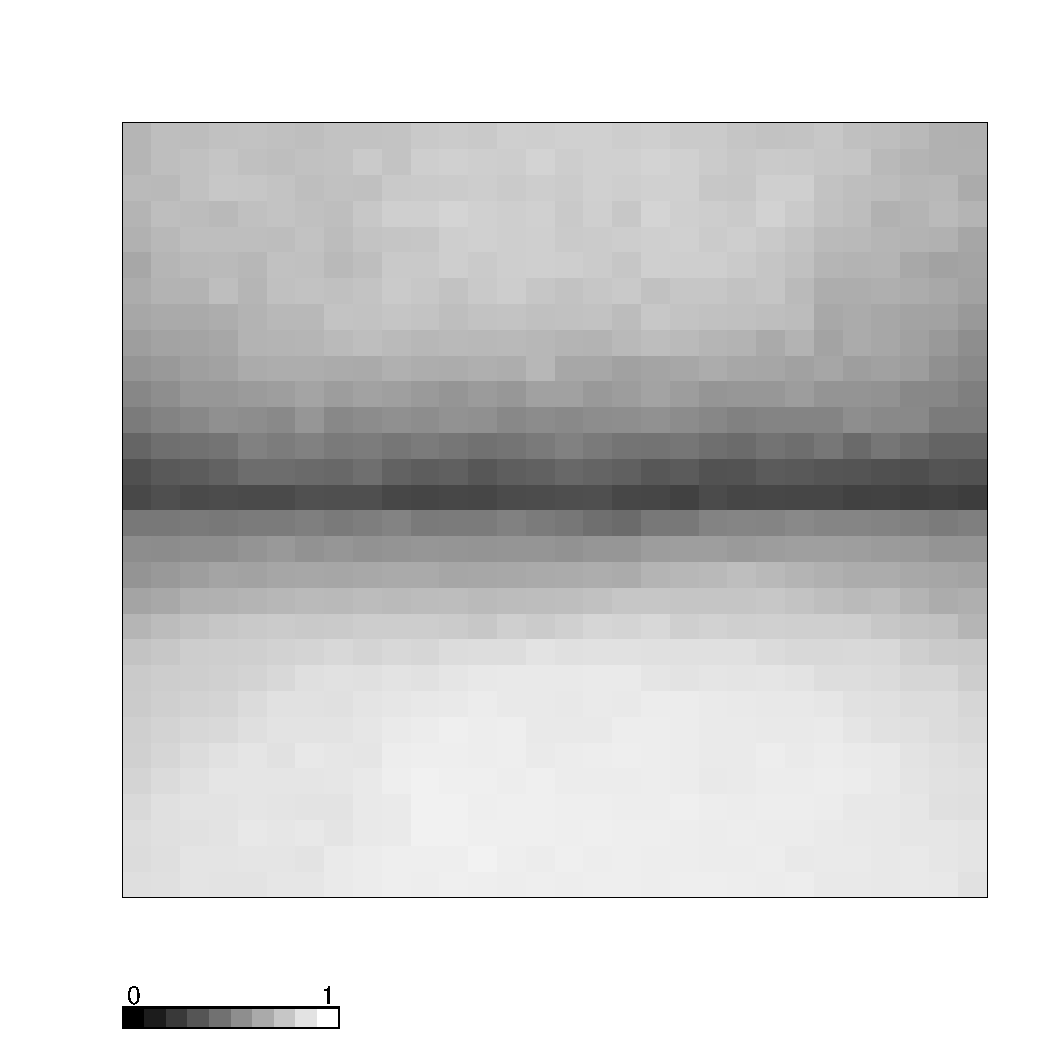
\includegraphics[width=3.1in]{../../figures/simulation/X1.coverage.pdf}
						\label{figX1:subfig1}
					}
					\subfigure[Selection frequency for $X_1$]{
						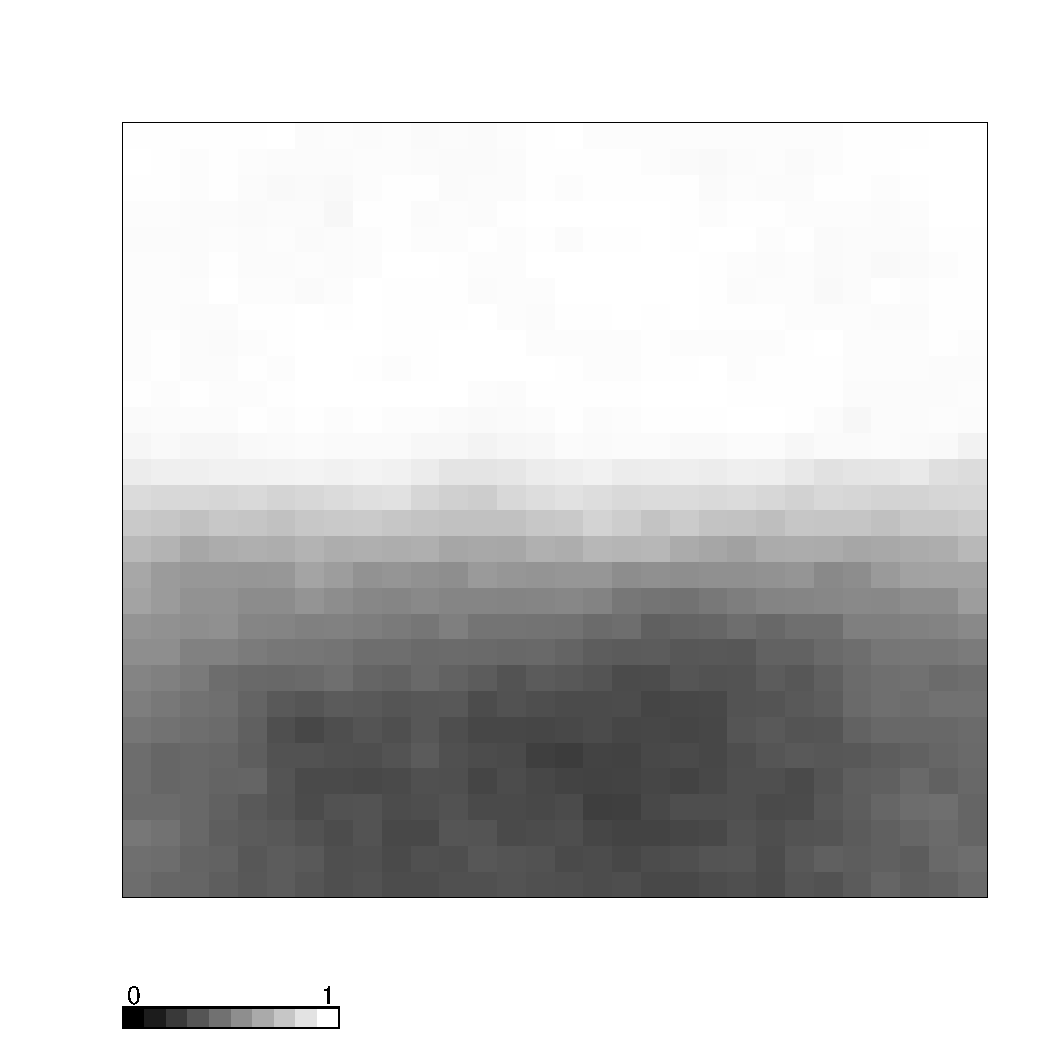
\includegraphics[width=3.1in]{../../figures/simulation/X1.selection.pdf}
						\label{figX1:subfig2}
					}
					\caption{Confidence interval coverage and selection frequency for $X_1$.\label{figX1}}
				\end{center}
			\end{figure}
					
					
			\begin{figure}
				\begin{center}
					\subfigure[Coverage of 95\% CI for $X_2$]{
						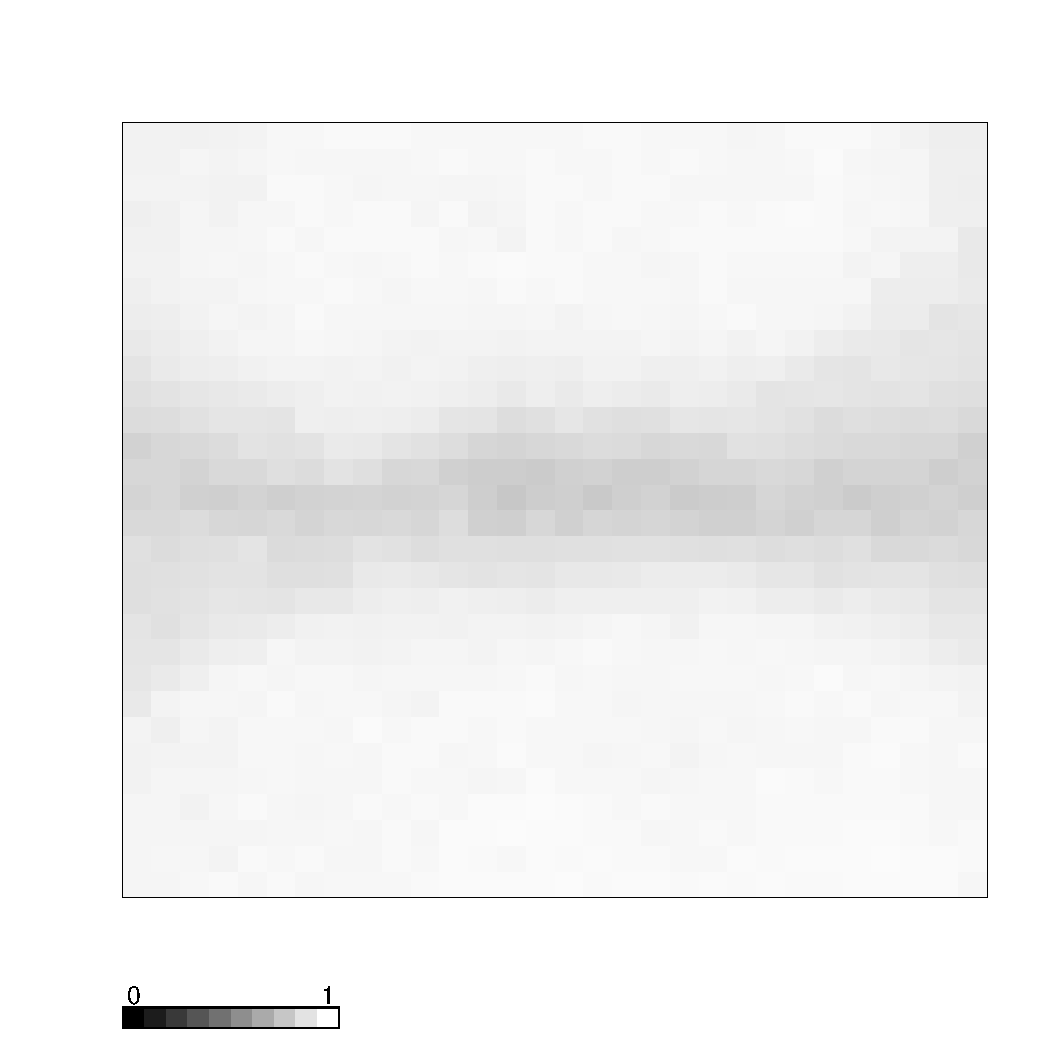
\includegraphics[width=3.1in]{../../figures/simulation/X2.coverage.pdf}
						\label{figX2:subfig1}
					}
					\subfigure[Selection frequency for $X_2$]{
						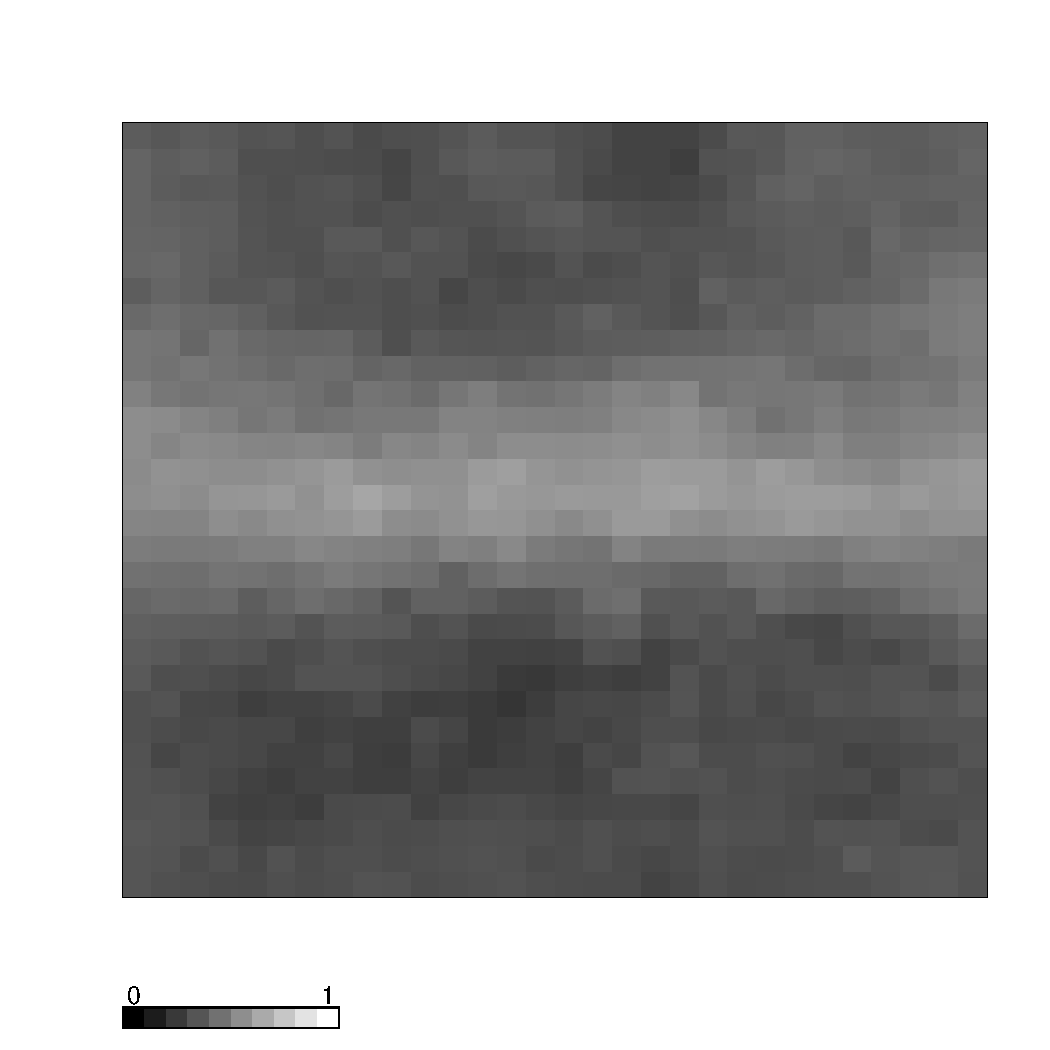
\includegraphics[width=3.1in]{../../figures/simulation/X2.selection.pdf}
						\label{figX2:subfig2}
					}									
					\caption{Confidence interval coverage and selection frequency for $X_2$.\label{figX2}}
				\end{center}
			\end{figure}
			
			
			\begin{figure}
				\begin{center}
					\subfigure[Coverage of 95\% CI for $X_3$]{
						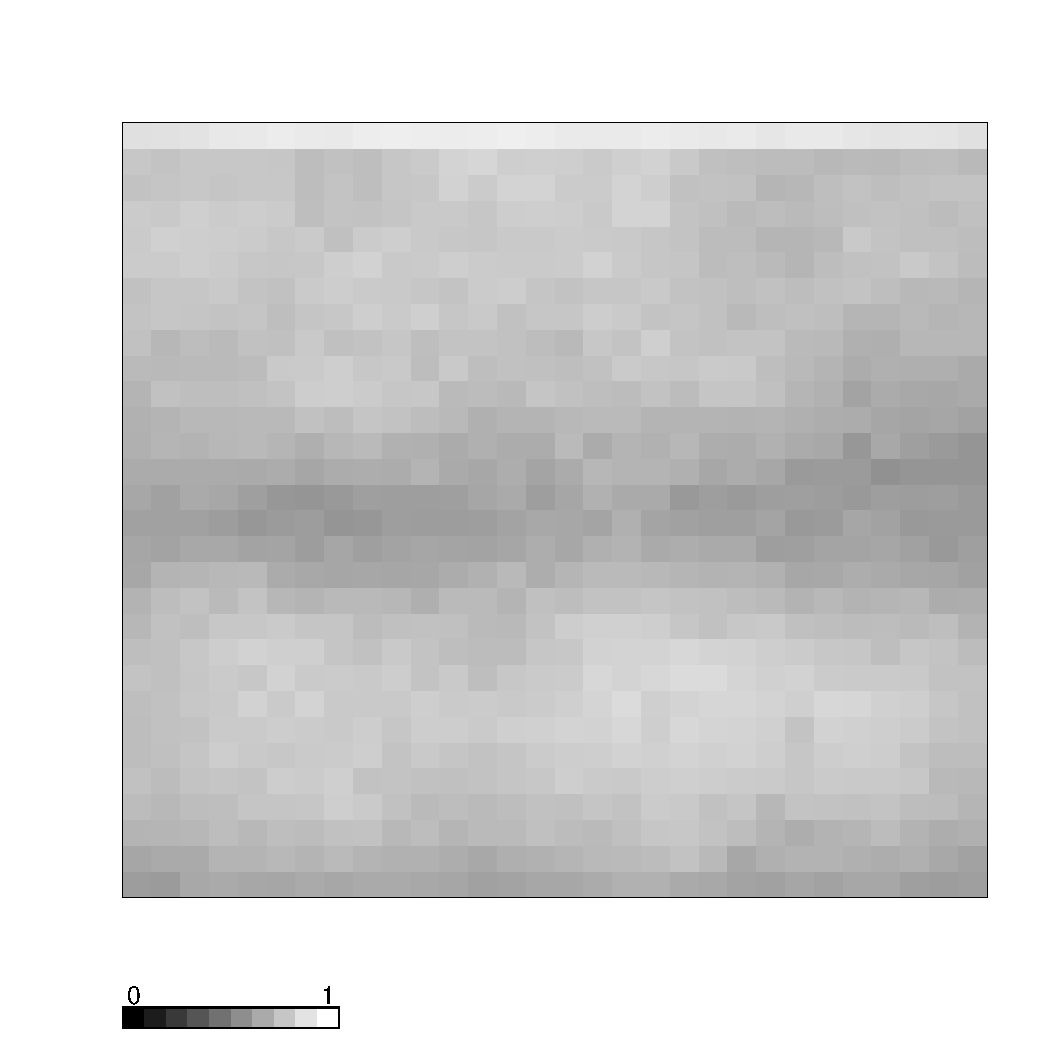
\includegraphics[width=3.1in]{../../figures/simulation/X3.coverage.pdf}
						\label{figX3:subfig1}
					}
					\subfigure[Selection frequency for $X_3$]{
						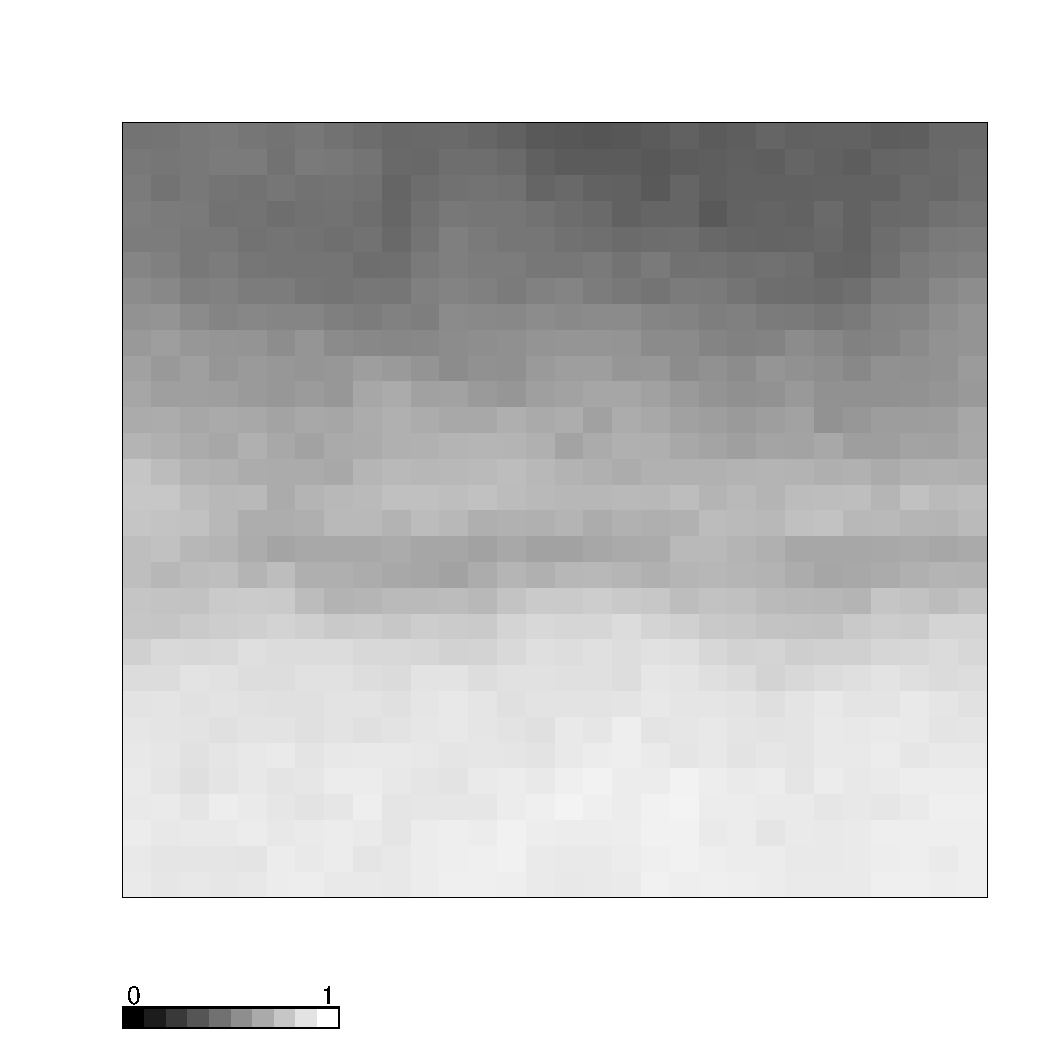
\includegraphics[width=3.1in]{../../figures/simulation/X3.selection.pdf}
						\label{figX3:subfig2}
					}									
					\caption{Confidence interval coverage and selection frequency for $X_3$.\label{figX3}}
				\end{center}
			\end{figure}
			
			
			\begin{figure}
				\begin{center}
					\subfigure[Coverage of 95\% CI for $X_4$]{
						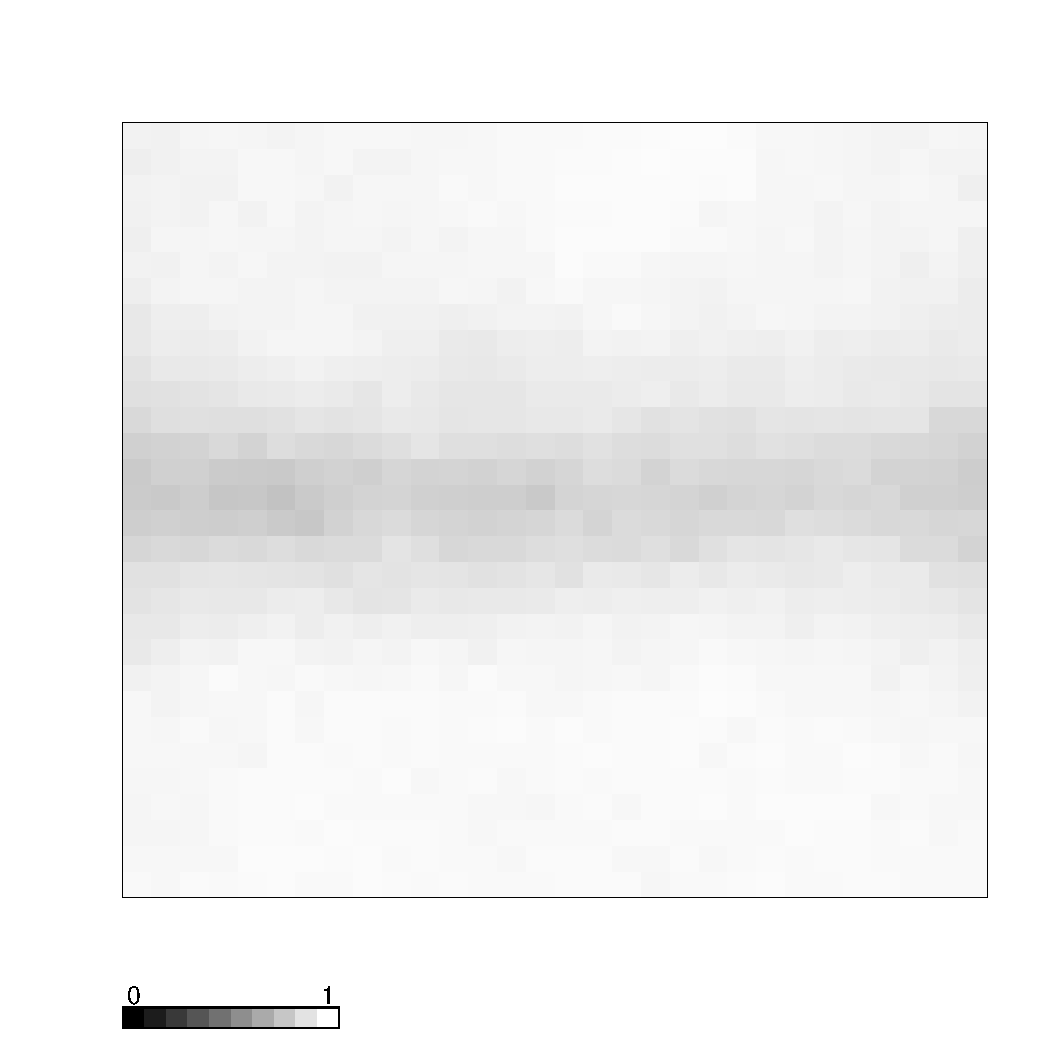
\includegraphics[width=3.1in]{../../figures/simulation/X4.coverage.pdf}
						\label{figX4:subfig1}
					}
					\subfigure[Selection frequency for $X_4$]{
						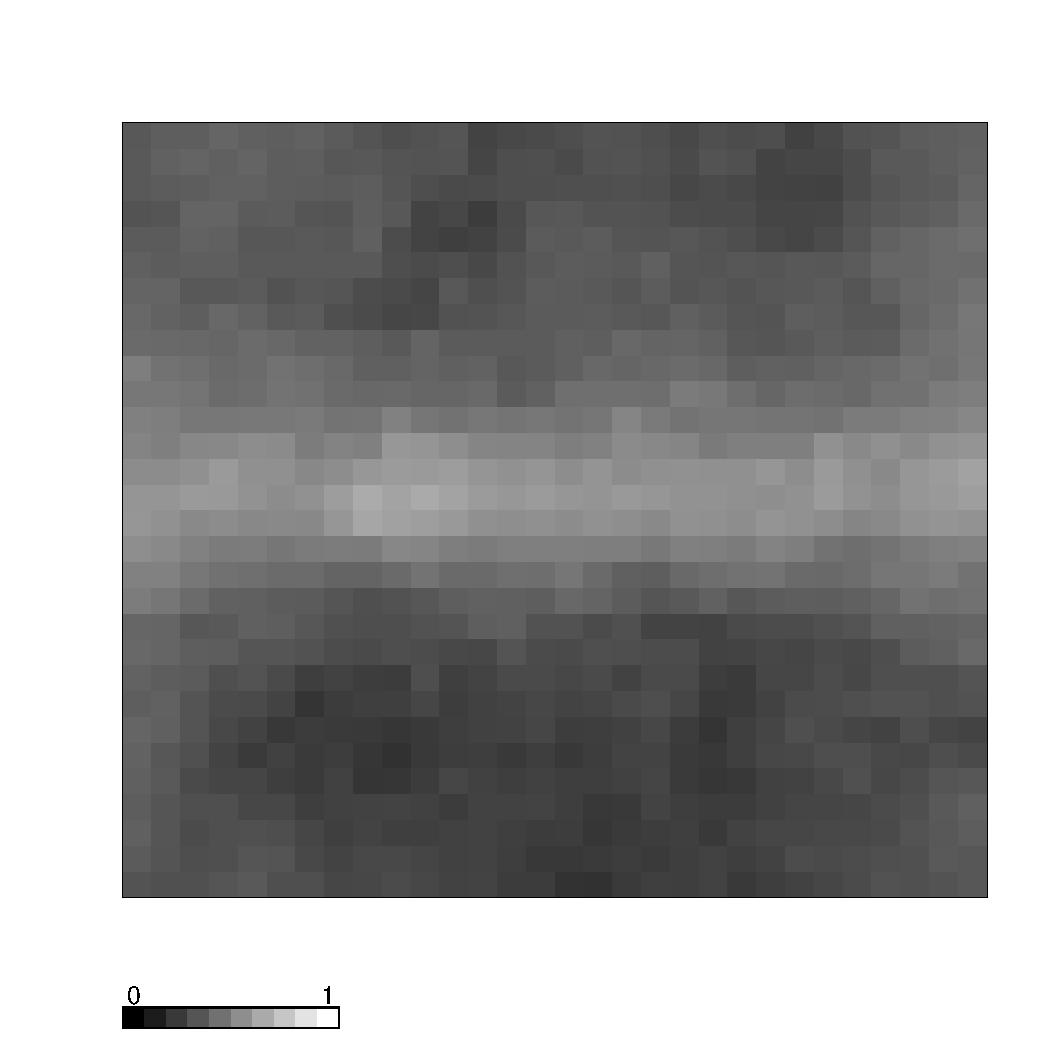
\includegraphics[width=3.1in]{../../figures/simulation/X4.selection.pdf}
						\label{figX4:subfig2}
					}									
					\caption{Confidence interval coverage and selection frequency for $X_4$.\label{figX4}}
				\end{center}
			\end{figure}
			
			
			\begin{figure}
				\begin{center}
					\subfigure[Coverage of 95\% CI for $X_5$]{
						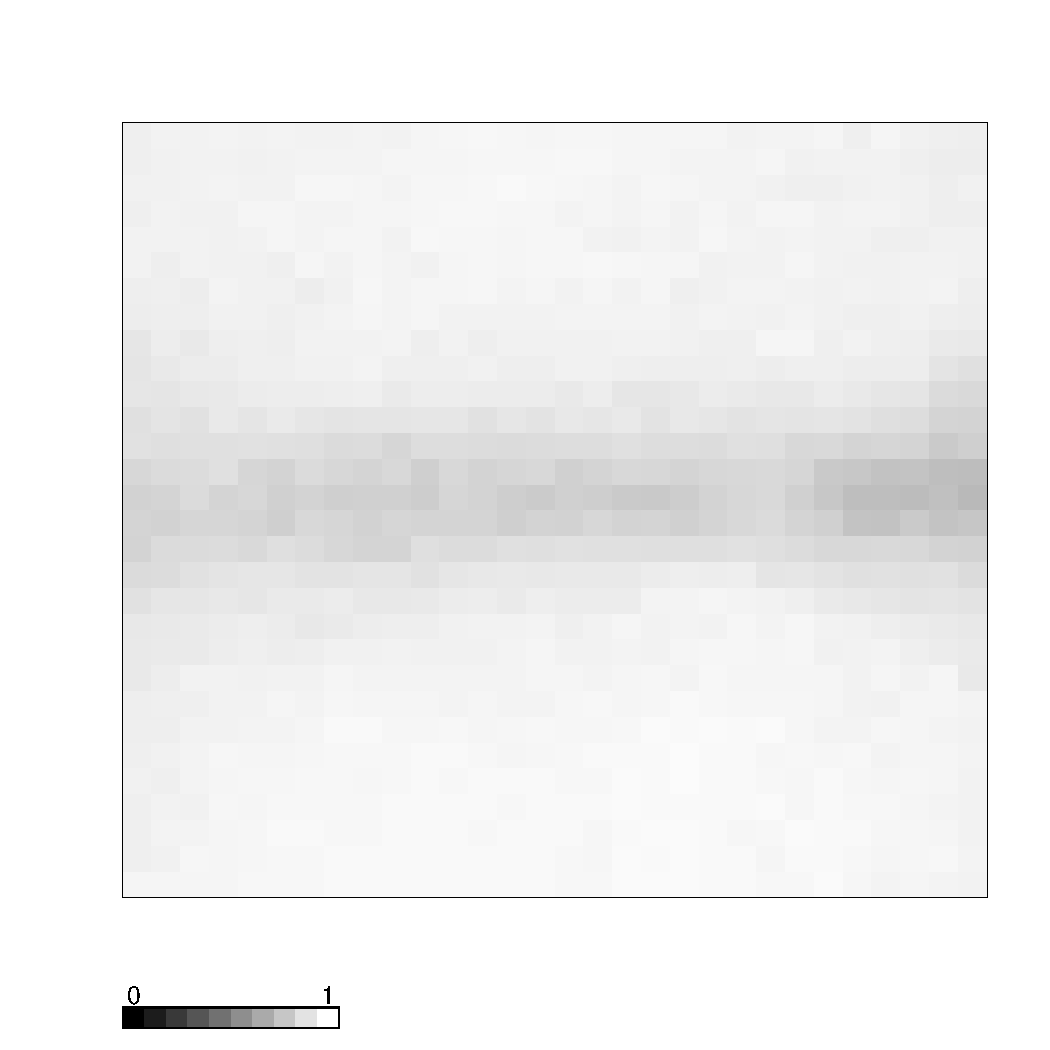
\includegraphics[width=3.1in]{../../figures/simulation/X5.coverage.pdf}
						\label{figX5:subfig1}
					}
					\subfigure[Selection frequency for $X_5$]{
						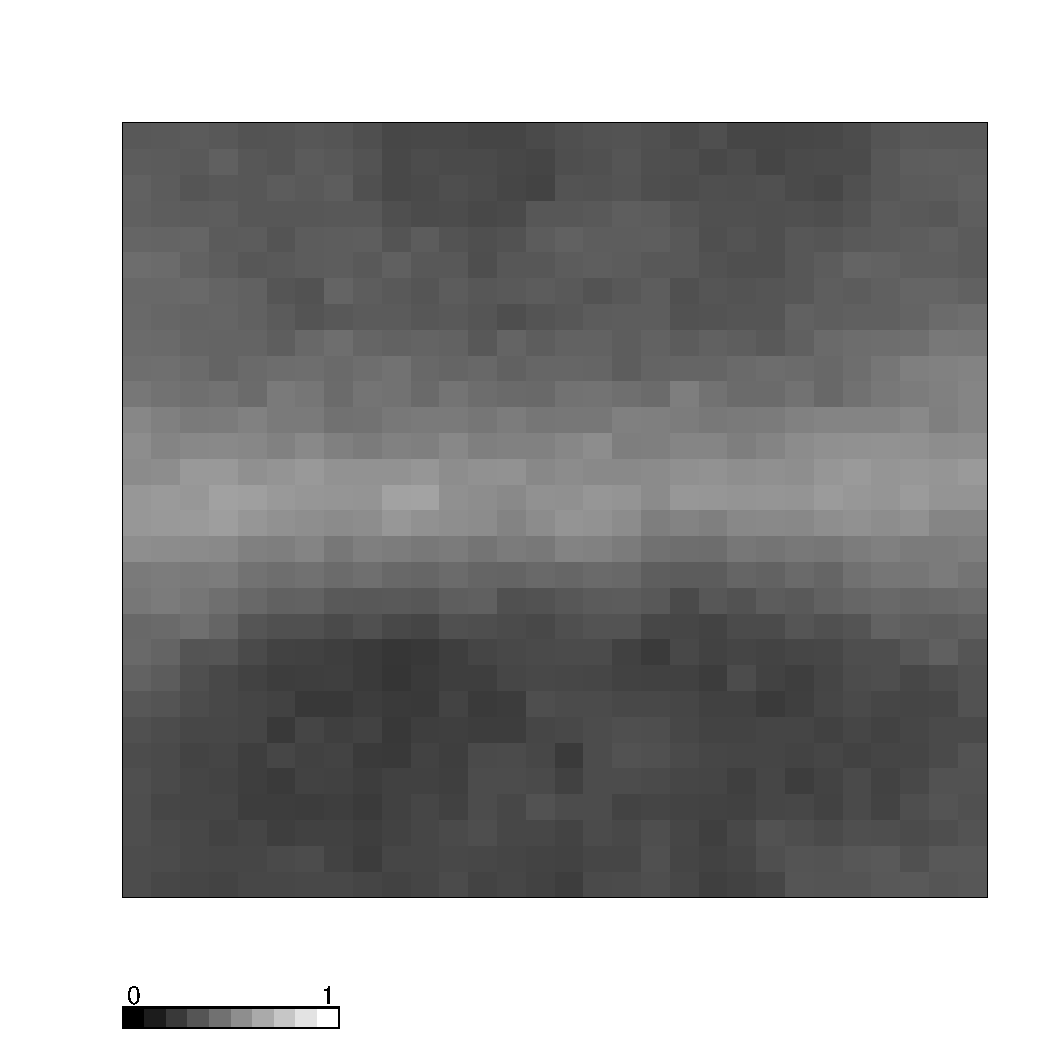
\includegraphics[width=3.1in]{../../figures/simulation/X5.selection.pdf}
						\label{figX5:subfig2}
					}									
					\caption{Confidence interval coverage and selection frequency for $X_5$.\label{figX5}}
				\end{center}
			\end{figure}
			
			
			\begin{figure}
				\begin{center}
					\subfigure[Coverage of 95\% CI for $Z$]{
						
\includegraphics[width=3.1in]{../../figures/simulation/Z.coverage.pdf}
						\label{figZ:subfig1}
					}
					\subfigure[Selection frequency for $Z$]{
						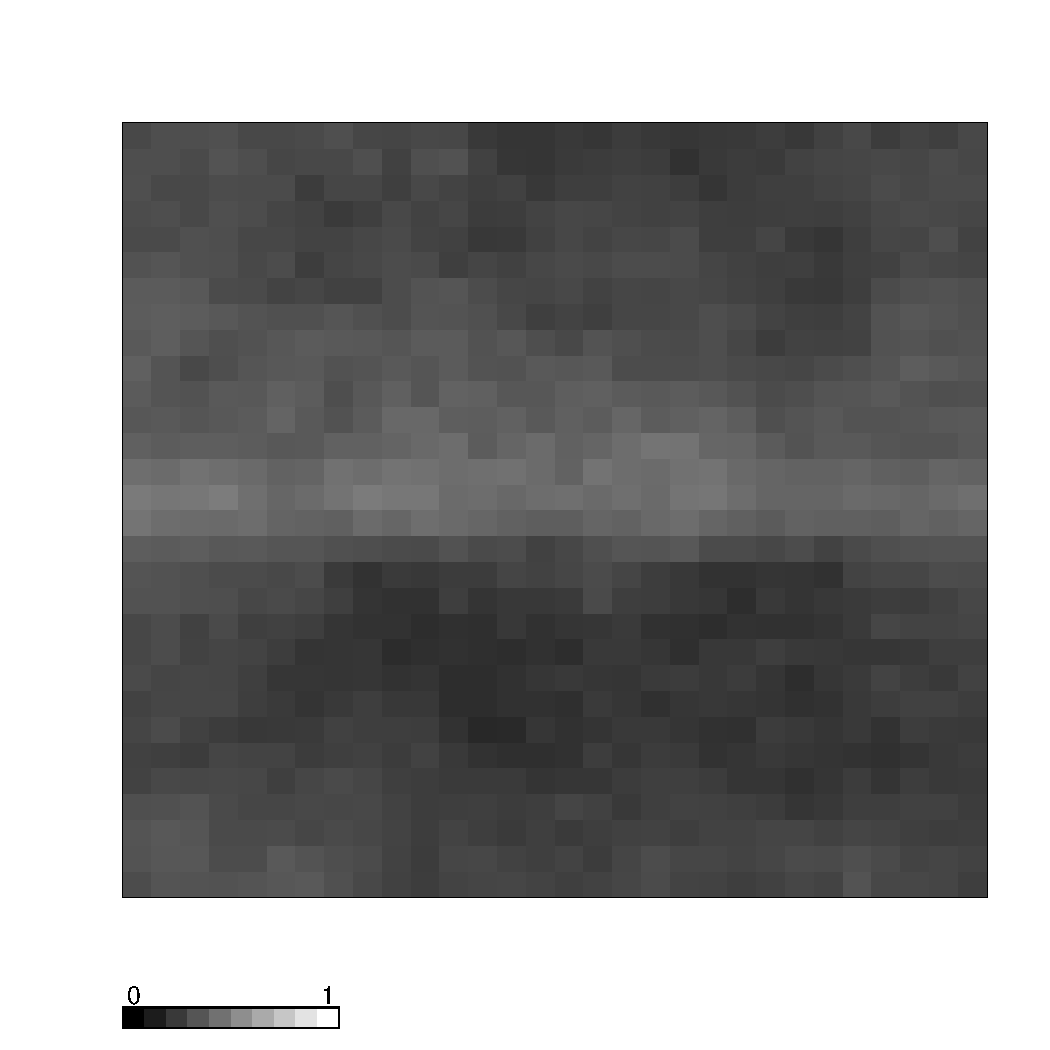
\includegraphics[width=3.1in]{../../figures/simulation/Z.selection.pdf}
						\label{figZ:subfig2}
					}									
					\caption{Confidence interval coverage and selection frequency for $Z$.\label{figZ}}
				\end{center}
			\end{figure}
			
			
			\begin{figure}
				\begin{center}
					\subfigure[Coverage of 95\% CI for intercept]{
						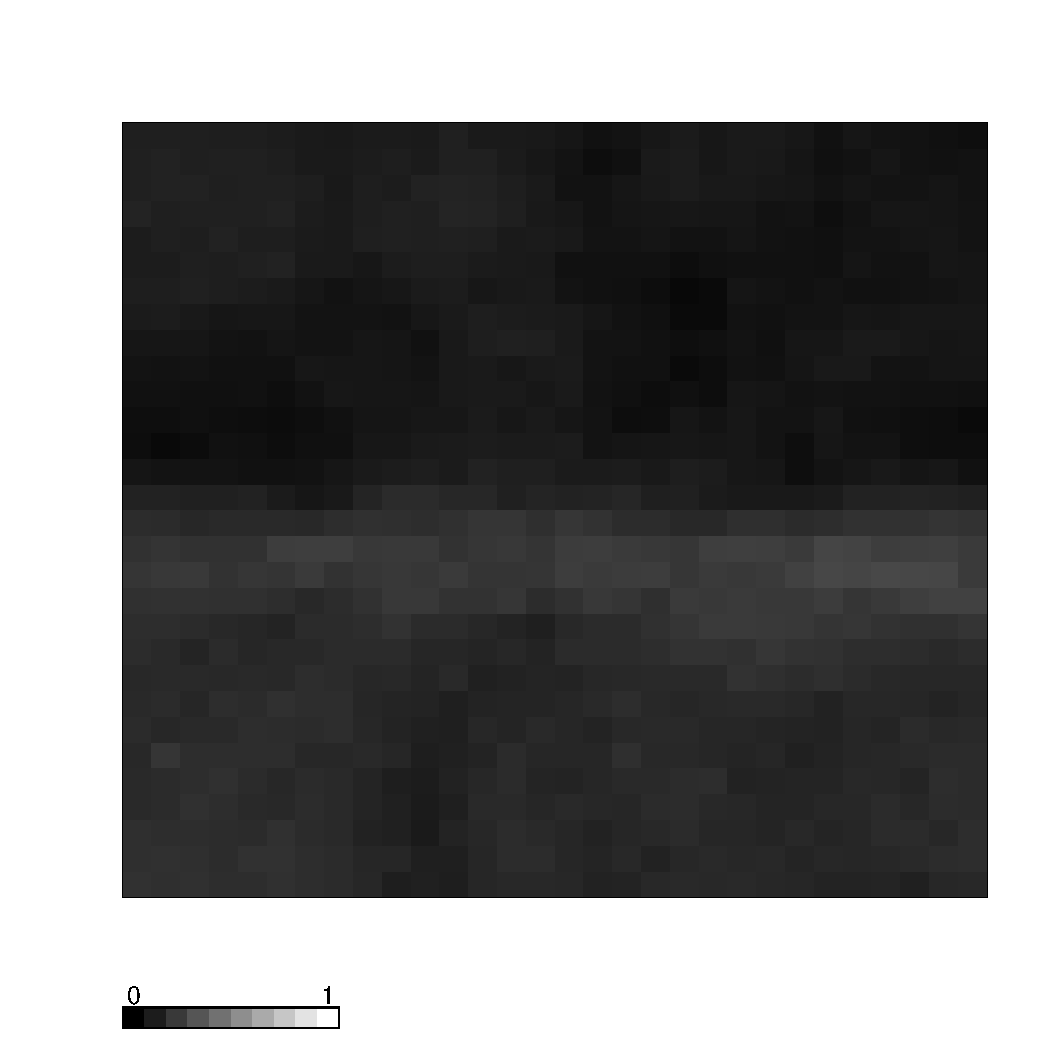
\includegraphics[width=3.1in]{../../figures/simulation/Intercept.coverage.pdf}
						\label{figIntercept:subfig1}
					}
					\subfigure[Selection frequency for intercept]{
						
\includegraphics[width=3.1in]{../../figures/simulation/Intercept.selection.pdf}
						\label{figIntercept:subfig2}
					}									
					\caption{Confidence interval coverage and selection frequency for intercept.\label{figIntercept}}
				\end{center}
			\end{figure}
			
			
			
			
			
		\subsection{Poverty data}
			\begin{figure}
				\begin{center}
					\includegraphics[width=5in]{../../figures/poverty/pag.estimate.pdf}
					\caption{Estimated coefficient surface for pag.\label{fig:pag}}
				\end{center}
			\end{figure}
					
					
			\begin{figure}
				\begin{center}
					\includegraphics[width=5in]{../../figures/poverty/pex.estimate.pdf}
					\caption{Estimated coefficient surface for pex.\label{fig:pex}}
				\end{center}
			\end{figure}
						
			
			\begin{figure}
				\begin{center}
					\includegraphics[width=5in]{../../figures/poverty/pman.estimate.pdf}
					\caption{Estimated coefficient surface for pman.\label{fig:pman}}
				\end{center}
			\end{figure}
						
			
			\begin{figure}
				\begin{center}
					\includegraphics[width=5in]{../../figures/poverty/pserve.estimate.pdf}
					\caption{Estimated coefficient surface for pserve.\label{fig:pserve}}
				\end{center}
			\end{figure}
						
			
			\begin{figure}
				\begin{center}
					\includegraphics[width=5in]{../../figures/poverty/pfire.estimate.pdf}
					\caption{Estimated coefficient surface for pfire.\label{fig:pfire}}
				\end{center}
			\end{figure}
						
			
			\begin{figure}
				\begin{center}
					\includegraphics[width=5in]{../../figures/poverty/potprof.estimate.pdf}
					\caption{Estimated coefficient surface for potprof.\label{fig:potprof}}
				\end{center}
			\end{figure}
			
			
			
			\begin{figure}
				\begin{center}
					\includegraphics[width=5in]{../../figures/poverty/pwh.estimate.pdf}
					\caption{Estimated coefficient surface for pwh.\label{fig:pwh}}
				\end{center}
			\end{figure}
						
			
			\begin{figure}
				\begin{center}
					\includegraphics[width=5in]{../../figures/poverty/pblk.estimate.pdf}
					\caption{Estimated coefficient surface for pblk.\label{fig:pblk}}
				\end{center}
			\end{figure}
						
			
			\begin{figure}
				\begin{center}
					\includegraphics[width=5in]{../../figures/poverty/phisp.estimate.pdf}
					\caption{Estimated coefficient surface for phisp.\label{fig:phisp}}
				\end{center}
			\end{figure}
						
			
			\begin{figure}
				\begin{center}
					\includegraphics[width=5in]{../../figures/poverty/metro.estimate.pdf}
					\caption{Estimated coefficient surface for metro.\label{fig:metro}}
				\end{center}
			\end{figure}
			


			
\bibliographystyle{plainnat}
\bibliography{../references/gwr}

\end{document}  